\documentclass[10pt]{report}
\usepackage{graphicx}
\usepackage{a4}
\usepackage{url}
\usepackage{fullpage}

% Report template authored V. Sorge, adapted S. Vickers.

\title{% This is the title of your document
{\normalsize Software Workshop Team Java (06-08165) 2010/11, Dr. E. Thompson}\\[2cm]
Project Report:\\
Space Runner Game}
\author{Team B3:\\
Daniel Cecil\\
Jere Ketonen\\
David Saunders\\
Michal Staniaszek
}

\begin{document}
\maketitle
\chapter*{Work Breakdown}
\label{work-breakdown}

\thispagestyle{empty}

% Obviously these need discussing and changing....
{\small

\noindent\begin{tabular}{|l||l|l|l|l|l|}\hline
  \textbf{Coding} & \textbf{Daniel} & \textbf{Jere} & \textbf{David}
 & \textbf{Michal} \\\hline\hline
 Datastructures & Contribution: 100\% & 0\% & 0\% & 0\%\\\hline
 \ldots & \ldots & \ldots & \ldots & \ldots \\\hline
\end{tabular}\vspace*{1cm}

\noindent\begin{tabular}{|l||l|l|l|l|l|}\hline
  \textbf{Report} & \textbf{Daniel} & \textbf{Jere} & \textbf{David}
 & \textbf{Michal}\\\hline\hline
 Introduction & Chapter~\ref{cha:introduction}: 100\% & 0\% & 0\% & 0\%\\\hline
 \ldots & \ldots & \ldots & \ldots & \ldots \\\hline
\end{tabular}

}     % This is the "}" that matches the "{" before "\small"

\tableofcontents
\thispagestyle{empty}

\begin{abstract}
  You should write a one-page abstract written as an ``Executive Summary''. It
  should be written for someone who is familiar with the Team Java module, so
  that there is no need for background or generalities. Rather, you should
  explain what is special about your project, and what you claim to have
  achieved. (One page maximum.)
\end{abstract}


\chapter{Introduction}
\label{cha:introduction}

This aim of this report is to give a overview of the team Java work we did for 11 weeks on a Space Shooter game and how it progressed from an idea on paper to a functional program.
It will be broken into sections covering important details on the design process, the way we worked and put the project together, the problems we faced, how we over came those problems and how we could improve the project futher with more time and resources.


Give a brief overview and guide the reader to the important points
in the remaining sections.

This template for your report also contains some examples of how to use some
{\LaTeX} elements and commands. In particular, there are examples for tables,
how to include figures, and various environments for bullet points or
enumerations.

For further information (and here is how to do a bullet list):
\begin{itemize}
\item look on the Team Java web page,\\
\url{http://www.cs.bham.ac.uk/internal/courses/team-java/current}\\
  (Click on ``Guidance''.)
\item google ``latex''
\item look at the \LaTeX book \cite{latex}
\end{itemize}


This is how to do numbered lists:
\begin{enumerate}
\item First point
\item Second point
\item \ldots
\end{enumerate}

This is how to do sections:

\section{Some topic}\label{some}

\section{Another topic}\label{another}

If you set a label with the \texttt{label} command, you can then use
the \texttt{ref} command to refer to that section -- e.g.
section~\ref{some}. This means you don't need to know about section
numbers. Note that \texttt{\~} means a space that cannot be broken
across lines.
 % needs doing...
\chapter{Requirements}
\label{cha:requirements}
\section{Functional User Requirements}
\label{sec: functional}

This section outlines the functional requirements which the system will be tested against. Functional requirements are what the system is expected to do and how to user interacts with the software. Each requirement is split into sub-requirements for ease of understanding and clarity.

\begin{enumerate}
\item \textbf{The human player is able to control one's spaceship}
\\* This is a core requirement needed to be able to play the game successfully in at least a single player mode without any crashes or bugs.
\begin{enumerate}
\item The user is able to use either a mouse or the keyboard's arrow keys to move the spaceship.
\item The user's spaceship is able to move freely along the x and y coordinates but not leave the frame's boundaries.
\item The user will be able to hold more than one key for diagonal movement where the movement speed much be normalised.
\item The user's spaceship will be able to be represented graphically on the screen.
\end{enumerate}

\item \textbf{The human player will be able to shoot}
\\* The aim of the game is to enable the user to destroy enemy ships and therefore shooting is a must-have requirement of the game.
\begin{enumerate}
\item The user will be able to shoot by tapping or holding the spacebar or the mouse button (left click).
\item The user's spaceship will have a type of weapon to use, this can be changed during the game (if implemented - dependant on future requirement).
\item The user's shot will follow a set path forwards (negative y-coordinate movement).
\item Shots which leave the frame's boundary will be removed from the game state.
\end{enumerate}

\item \textbf{Enemies will be created to be destroyed by the user}
\\* This is a core functional requirement that needs to be implemented to enable the user to progress through the game by shooting down opposing units.
\begin{enumerate}
\item Enemies will be spawned at set locations on the screen.
\item Enemy units are to have a set health limit.
\item Enemies will be able to be shot by any user spaceship.
\item Enemies are to be distinguishable from friendly user spaceships by using different shapes or graphics.
\item The enemy unit's health will be decreased when a user's shot collides with the enemy.
\item Enemy's will 'die' once all their health have been depleted.
\end{enumerate}

\item \textbf{Enemies are to be able to return a level of resistance}
\\* This requirement is needed to make the game more interesting by introducing the possibility of a player 'death'
\begin{enumerate}
\item Enemies are able to return shots towards the human players with the use of different weapons.
\item Enemies are able to move in certain paths (zig-zag, diagonal, straight, side-to-side).
\item If the player collides with an enemy the player will 'die'
\item 'Boss' enemies are to be introduced which fire more shots and have more health.
\end{enumerate}

\item \textbf{The game is to run continuously with set events occurring at regular intervals}
\\* This requirement ensures the game runs smoothly and that something will always happen. For example, to stop the incidence of no more enemies being spawned (so the game is playable).
\begin{enumerate}
\item The game is to implement a Timer class.
\item Enemies will always be spawned at set intervals during the game. These can be changed to be more or less frequent (if future requirement is implemented).
\item Each tick of the timer will move enemies, player units (depending on user input) and projectiles.
\item The game panel will be redrawn at every tick of the timer.
\end{enumerate}

\item \textbf{The game will be able to be multiplayer across the network}
\\* This requirement is necessary to fulfil the assessment criteria allowing for a second human user to play in co-operative mode with each other against the computer enemies.
\begin{enumerate}
\item Each human user will be able to select whether they will act as the host or the client PC.
\item Clients will be able to enter the Host's IP address to connect.
\item The host's game will start immediately after selection with clients dropping into the game at a set spawn point.
\item The game must be able to support at least two human players and a maximum of eight players (7 clients).
\item All users must be connected to the same LAN network.
\item All users must have similar game information on their screens (player, enemy and projectile positions).
\item With each tick of the timer (requirement 5) each player's screen will be updated with network data from the host.
\end{enumerate}

\item \textbf{The game must have a terminating clause}
\\* This requirement ensures that the game will end at some point.
\begin{enumerate}
\item Once a player's health has been depleted, that unit will 'die' and be removed from the game allowing other player's to carry on playing.
\item If a player collides with an enemy unit they will also 'die'
\item The player's score will be displayed on termination and if high enough will be recorded in a high scores table.
\end{enumerate}

\item \textbf{The game will include a Graphical User Interface (GUI)}
\\* This allows all users to be able to start the necessary game type as well as actually play the game with the information displayed on the screen.
\begin{enumerate}
\item The game will run from a single frame.
\item Panels are to be added to the frame: Menu, Game, Gameover.
\item The Menu Panel is to feature buttons corresponding to various game types and options.
\item The Menu Panel is to be accessible from within the game (Esc key).
\item The Game is to be able to be paused using the 'P' key.
\item The window is to be resizable allowing for full-screen play.
\item The Game Panel is to feature a scrolling 'star-like' background (black with white stars).
\item The game objects (players, enemies and projectiles) are to be represented by shapes or sprites (graphics).
\end{enumerate}

\end{enumerate}


\subsection{Attributes}
\label{sec: req_attributes}

\noindent\begin{tabular}{| l || p{6cm} | p{7cm} |}\hline
  \textbf{Attribute} & \textbf{Requirement No.} & \textbf{Comment}  \\\hline\hline
  Status & All & Approved - development started \\\hline
 Priority & 1, 2, 3, 4abc, 5, 6, 7, 8abch  - Mandatory. &  Mandatory requirements must be implemented.\\
 & 4d, 8defg - Important & \\\hline
 Effort & All & Deadline for code: 22/03/11 (10 weeks). Estimated 40 person-weeks for first release. \\\hline
 Risk & All & Medium probability of risk occurring. Large impact if assessment is not complete. High risk with networking code due to lack of experience. \\\hline
 Target Release & 1, 8a, 8h & v0.1 \\
 & 2 & v0.2 \\
 & 3b-f & v0.3 \\
 & 4, 5, 7 & v0.4 \\
 & 3a, 8b-g & v0.5 \\
 & 6 & v0.6 \\\hline
 Assigned To & All & 4 x Team Members. Requirements and tasks to be distributed at weekly meetings. \\\hline
\end{tabular}\vspace*{1cm}


\section{Non-functional User Requirements}
\label{sec: non-functional}

This section outlines the non-functional requirements. These requirements relate to the quality of the product and testing requires opinions and qualitative methods rather than quantitative feedback. The project has been split into different categories of requirement.

\paragraph{Usability} 
\begin{enumerate}
\setcounter{enumi}{8}
\item \textbf{To provide a simple, easy to use system in order to play the game}
\begin{enumerate}
\item A novice to the game should be able to gain understanding and play the game within 10 minutes of first playing.
\item Expert gamers should be able to grasp game concept within 1-2 minutes of playing.
\item The game should have a clean look and feel.
\item The user should feel in control of their spaceship with smooth movement and quick reactions.
\item The menu should have a standard, organised layout with minimal pages
\item The game should have a professional look
\end{enumerate}
\end{enumerate}
A user manual or help pages are not required due to the limitations on time for the assessment and the game itself is believed to be simple enough for most people to be able to understand.

\paragraph{Efficiency}
\begin{enumerate}
\setcounter{enumi}{9}
\item \textbf{The game should be constantly quick to respond}
\begin{enumerate}
\item The game should run at a constant quick speed without any lag.
\item The user's input should have an almost instant effect on the game.
\item Network play should be stable for 95\% of the time.
\end{enumerate}
\end{enumerate}

\paragraph{Dependability}
\begin{enumerate}
\setcounter{enumi}{10}
\item The game should run first time, all of the time as single player or host.
\item Network clients should be able to drop-into the host's game within 5 seconds.
\end{enumerate}

\paragraph{Environmental}
\begin{enumerate}
\setcounter{enumi}{12}
\item The game should run on the platforms detailed in the below section (system requirements).
\end{enumerate}

\paragraph{Development}
\begin{enumerate}
\setcounter{enumi}{13}
\item The project should be developed using appropriate software engineering practises within the time frame for the assessment.
\item The project must be written in the Java programming language.
\end{enumerate}

\paragraph{Operational}
\begin{enumerate}
\setcounter{enumi}{15}
\item The multiplayer game must be able to run on any LAN with the IP addresses given.
\item High scores will remain stored in each copy of the game until they are overridden by a higher score.
\end{enumerate}

\section{System Requirements}
\label {sec: system_requirements}
This section details the requirements and physical devices needed to play the game successfully.

\begin{enumerate}
	\item The game is to be written in the Java programming language.
	\item All user PCs will need to follow the system requirements for Java 6
	\begin{enumerate}
	\item Windows 7, Vista, XP, 2000, Server 2008, Server 2003. All 32 and 64-bit operating systems
	\item Mac OS X
	\item Most Linux distributions
	\item Solaris
	\end{enumerate}
\item Keyboard and Mouse are required (with Western layout)
\item For multiplayer, all users will need to be connected to a local area network (LAN) at least
\item Monitor and graphics card with at least a resolution of 800 x 600 
\end{enumerate}

\section{Future Requirements}
\label{sec: future_requirements}
Requirements 1 to 17 are aimed at the first release which is as far as the project is aimed to go. However if the project is ahead of schedule the progress will be re-evaluated and requirements from this list will be introduced depending on complexity and remaining time and resources available.
\begin{itemize}
\item Power Ups
	\begin{itemize}
	\item Increased health
	\item Increased shot damage
	\item Enemies freeze
	\item Move quicker
	\end{itemize}
\item Boss Fights
	\begin{itemize}
	\item Enemy unit with lots of health - harder to kill
	\item Enemy has greater weapons
	\item Enemy does not move off screen (has to be killed)
	\end{itemize}
\item Different Weapons
	\begin{itemize}
	\item Greater damage
	\item Single-shot
	\item Multiple direction shooting
	\end{itemize}
\item Increasing Difficulty
	\begin{itemize}
	\item Enemies spawn more often in larger numbers
	\item Enemies have greater damage
	\item Enemies have greater health
	\item Enemies shoot more often
	\item More boss fights
	\end{itemize}
\item Background music added
\item Endless mode (player respawns)
\end{itemize}
\chapter{Design}
\label{cha:design}

This section is crucial. Describe the overall structure of your
program at a suitably high level of abstraction. For instance, UML
diagrams or informal box-and-arrow diagrams can be used to describe
program structure. Be sure to describe the MVC structure used. Note
that code listings or screenshots are not appropriate here. An
important point is how you have divided the project into modules
that different team members can work on, and how these are then
integrated. For example, you could use interfaces to describe a
clean boundary between modules, so that some team members use the
functionality provided by the interface, while another team member
implements it. Bear in mind Software Engineering principles of good
design like coherence and coupling.

\section{Release Plan}
\label{sec: release_plan}
This section outlines the proposed release plan of the project. It has been decided that the project will take the incremental approach of software development with acceptance testing taking place at each stage. The six internal releases will be implemented consecutively to bring the project to the first public release within the 10 week timeframe.

\begin{itemize}
\item \textbf{Version 0.1:} Basic player spaceship (Java shape) on screen with controls and movement.
\item \textbf{Version 0.2:} Basic shooting from the player's spaceship.
\item \textbf{Version 0.3:} Static enemies on the screen, player able to shoot the enemy and score incremented.
\item \textbf{Version 0.4:} Enemies have movement with the use of paths, are able to shoot back and collide with players.
\item \textbf{Version 0.5:} Background scrolling, enemies are spawned at regular intervals at set points using a timer.
\item \textbf{Version 0.6:} Multiplayer networking implemented.
\end{itemize} This brings the project to the first public stable release which satisfies the requirements for the assessment. It time is available certain future requirements (section \ref{sec: future_requirements}) towards the second public release.

\section{Class Design}
\label{sec: class_design}
Below shows a diagram of how the project is to be organised in terms of classes and packages (dotted lines show packages).
\begin{figure}
 \centering
 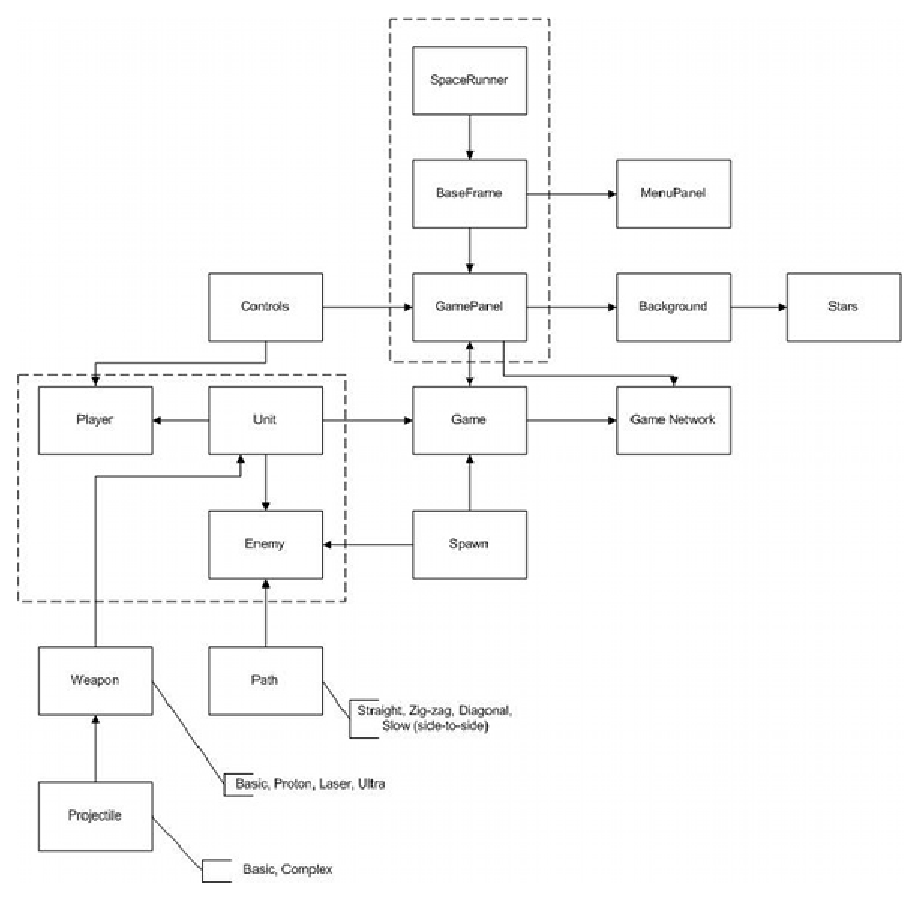
\includegraphics{class_diagram_small.eps}
 \caption{Proposed class diagram for the project}
 \label{fig: class_diagram}
\end{figure}

\section{Implementation}
\subsection{GUI and Controls}
The GUI was written using the standard JFrame and JPanel layout. A menu and a game panel were embedded inside the JFrame using a panel with a CardLayout. The menu and panel are part of the card layout, and can therefore be switched to very easily by referring to the name given to the CardLayout when each panel is added. There were some problems implementing a switching method to switch out the game and menu when either was required. Since the GamePanel is controlled by a timer, it is not possible to throw exceptions out. Therefore, another method was devised, by which the frame would call a method in the currently active panel to check if a `switch' flag was set. Based on this flag, the frame would change the panel that was currently being displayed, along with performing relevant actions. For example, when the menu is accessed while playing the game, the game has to be paused, and so the frame accesses a variable in the GamePanel which controls whether the game logic is progressing or not.
\subsection{Menu}
The menu is composed of simple objects such as rectangles that switch out using card panels. These card panels allow for easy switching of panels when an action is performed such as for our game when the user clicks to start a single player game. The way the panel detects what the user wants us by using mouse listners and checking if the mouse is within the bounds of the rectangle when the mouse button is clicked. Once clicked the panel will switch out to the coresponding panel action that was designated as the action of the "on click" of the rectangle. Another thing to note is that when escape is pressed suring game play the game will pause and switch the panel out back to the menu where the user can then either start a new game or resume the current game.
\subsection{Controls}
The controls for the game were implemented by using mouse and key listeners as to allow the user the choice of input method. The main way the controls work is by first detecting if the keyboard or mouse is being used and then using the apropriate method. For the mouse it would get the current pointer location and move the ship to that location on screen as well as listening for mouse button presses to triger the shooting method. The keyboard worked by detecting which key was being pressed and setting a boolian value to be true, this allowed the user to press multiple keys at once to move the ship diagonaly while also shooting. The control class was embeded into the game panel class so it ran when ever the game was started. Using the boolian values from the control class then decided upon where the ship would move to and if it was shooting or not.
\subsection{Game Logic}
The game logic is run in a loop that is controled by the game timer. The timer decideds on the frame rate of the game which affects the speed of which objects such as projectiles can move. Also within the game logic loop major components to the game such as collision detection and array pruning are called from the logic method. This part of the came could be said to be the game core that calls all the neccesary methods.
\subsubsection{Overview}
The game logic was written as a part of the program that could be used easily without any knowledge of the actual processing going on inside. The game logic is made up of a series of arrays, each consisting of objects that are part of the game; spawns, players, enemies and projectiles. These arrays are modified by the game in order to update the current state of the game. The arrays can be accessed by any class via getter methods, and objects can be added and removed if necessary. The logic can also perform removal of objects on command using certain pruning methods which are described later. The game logic also has methods to move all objects on the screen to new positions. The objects inside the arrays are manipulated inside the game panel using the methods of the game class. After logic has been done on the arrays, the panel then draws the objects inside the arrays.
\subsubsection{Collision detection}
The collision detection is na\"{i}ve, and done in two separate stages. Collisions of enemies with player projectiles is done first, and then collisions of enemy projectiles with the player, and enemies themselves with the player. This method is quick, and is not particularly computationally intensive given the type of game that we have written. Whether a collision actually occurs or not is defined by using a rectangular `hitbox' which surrounds the unit or projectile. If the hitboxes overlap, then the damage that the bullet carries is transmitted to the unit, and if the unit's health drops to zero or below as a result, the unit is removed from the array. The projectiles is removed from the array when it collides with a player or enemy object. Doing this gives quite a realistic feeling---it is not usual that a projectile passes through an object. However, implementing weapons that travel through units would not be problematic either, given the structure of the code. In order to avoid concurrent modification problems, enemies and projectiles that must be removed from arrays must first be stored in a secondary arraylist, which is then used to remove objects from the original array once all of the collisions have been checked.
\subsubsection{Array Pruning}
So as not to overload the memory of the computer with a huge number of objects, the arrays in the game are pruned of projectiles and enemies that are no longer within the visible area of the screen. This is done by creating a rectangle the size of the frame window, with the same coordinate space, and then, avoiding concurrent modification, removing the objects whose locations are not within the bounds of the frame rectangle. This also means that less processing is necessary during collision detection, and there are fewer objects that must be dealt with.
\subsection{Game Entities}
\subsubsection{Units}
For the units, we defined an abstract class that would contain all methods that would be necessary to access the basic information about the unit such as health. The game contains two subclasses of the unit class, player and enemy. In each of these classes, there are some parts that are specific to the requirements of those objects. For example, enemies have a method to get the value in points for destroying them, and the player class has a method to increment the score for that player. Using an abstract class meant that the subclasses already had all the necessary methods for access, and only needed some simple additional methods that were specific to the type of unit, and this saved writing quite a lot of unnecessary code. Each enemy unit moves based upon a path. Paths consist of a single equation, along with some directional variables to determine the next position of a unit based on its current position. Each time the game logic is run, this method is called with the object's current location, and returns the location that the object is due to move to next. This sort of implementation of paths allows for a robust method of control for both enemies and projectiles, and can be used to create a variety of interesting path types relatively easily, which allows for good extensibility. These paths also mean that the speed of units and projectiles can be controlled by using some sort of speed variable to increase the multiplier on the default additions to the coordinates, which would be very useful if there were to be difficulty levels added.
\subsubsection{Weapons and Projectiles}
The weapon and projectile classes are fundamental to the gameplay of the game. The weapon class is an abstract class which is intended to allow for quick addition of new weapon types into the game. Each weapon has a fire method which causes the weapon to create a new arraylist containing a number of projectiles specified by the method. This means that it is simple to add new projectiles to the game logic from quite a high position based on object orientation. Once one has a reference to a unit, it is only necessary to get the reference of the weapon, and then add the return array of the fire method to the game logic when one wants to cause weapons to fire. Each weapon has a fire rate, which is used by the logic to determine whether the weapon's fire method should be called or not. This allows for precise control of the weapons firing.

Projectiles are very simple objects which move based on paths. Each projectile object contains some data about which player it was spawned from (if it was), and details about its damage.
\subsubsection{Spawns}
The Spawn class is used to create new enemies during the game. The game has seven different set spawn points at regular intervals along the top of the screen, these points are held inside an array within the Spawn class. The class is currently able to spawn three types of enemy units: default unit which is abstract so that future types of unit can be created, boss enemy which is harder to shoot as it has increased health and different weapons as well as moving along a different path and finally the basic enemy unit which makes up the majority of the game. The spawn methods are called on the Spawn object in the GamePanel class at regular intervals in the game cycle (timer). There are various different types of spawn options available:
\begin{itemize}
	\item Spawn 1 unit at a given point (0.8\% chance of it being a boss enemy).
	\item Spawn a given number of units at the same given point.
	\item Spawn a given number of units at the same random point.
	\item Spawn a given number of units at different (chance of it being the same) random point.
\end{itemize}
Each of these methods returns an ArrayList of Units which can then be drawn in the render method in the GamePanel class. The Spawn class is abstract and can be modified in the future to add new types of enemy, the frequency can be changed in the GamePanel of how often units are spawned too.
\subsection{Network}
Networking is based on a client-server principle. Upon choosing the multiplayer option in the menu, the player is given a choice of hosting or joining a game. Depending on the option chosen, the game panel is initialised with server or client object which perform different tasks. When a client connects to the server via an input IP address, the server receives a reference to the client, which it then stores in a map. This map is used to get references to clients when data has to be sent to them. With a map, it is easy to send either to all clients, or choose a specific client to send data to. Client connections are dealt with by a handler, which sits in its own thread and waits for connection attempts to the server. When a connection is received, the handler adds the connection to the server's map via the interface, and the client immediately begins receiving any data from the server. Each individual client is embedded inside a class which contains methods to perform specific actions such as sending data over the network. The client and server perform interactions by first sending a string containing some information about the message that is to be sent next, and then sending the message. This method of communication is facilitated by a listener which runs in its own thread and constantly listens for commands coming in. If a command is received, a method in the socket is called to execute the request. This well structured communication method means that all communication can be handled in the correct way for that particular command. The method by which data is communicated over the network is via game state objects, which contain all the data needed by the game to run correctly; all the arrays, and boolean variables representing whether the game is running or not, along with a few others. The game state is capable of doing some processing, in order to reduce the data that is transferred over the network. A client first receives data from the server, and then runs its logic on it, moving projectiles fired by all units, and moving the player location. Each loop, the current state of the game is made into a new game state. This game state is then compared against the game state that was received from the server at the start of the loop. All objects that are the same in both game states are ignored---only new objects and the player reference are passed to the server, which reduces load on the network and also makes it easier for the server to collate the data into a single new game state which combines data from all clients which are currently connected. The server takes the new amalgamated game state, performs logic on it, and then sends it out to all clients, and the cycle continues. This method, along with the client storage method means that clients can drop in and out of the game without any wait time. In order to facilitate the transfer of objects over the network, upon object creation, each object is given a reference which will allow checking of the objects even if they are duplicated later, which is necessary for the removal of old objects.
\subsection{Graphics}
Graphics is implemented using a map stored in the game panel class. This map is initialised upon loading of the game with images from the relevant locations. Each object which must be drawn has an image reference string, which refers to the string that the image was added to the map with. When the object is drawn, the image reference is used to retrieve the image for that particular object, which is passed to the draw method of the object, which then draws it. Using this method meant that it was not necessary to pass images over the network, which would greatly slow communication due to the relatively large size of images. However, this method could, in theory, lead to the modification of the image files which are used to draw objects. In actuality, this will have no real effect on gameplay, since the size of the images are not at all considered when processing game logic.
\section{GUI Design}
\label{sec: gui_design}
The GUI will be fairly simple and initially the on-screen components will be made up of shapes (Java objects). The initial sketches are shown below which were created in the first week of development to aim understanding of the project.\\
\begin{center}
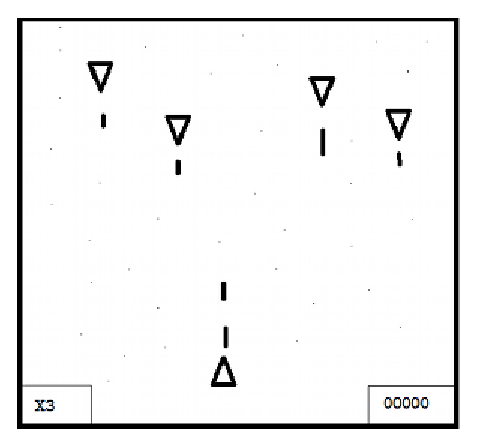
\includegraphics{GUI1.eps}
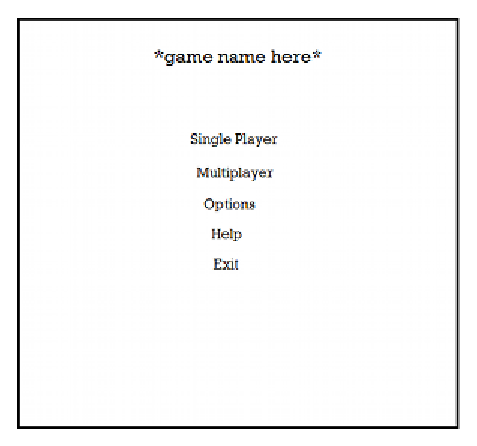
\includegraphics{GUI2.eps}
\end{center}
The menu screen (right) will have buttons that allow the user to select different types of game play, for example single or multi-player, as well as being able to exit the game or select different options. The menu is also accessible from within the game using the Esc key.\\\\
The game is to be implemented in a single window (frame) with different panels added (i.e. menu and game panels). The frame is to be resizable (including the layouts of ships) to allow the user to change the game from the default size.\\\\
In the Game Panel (left) the objects are represented as shapes. These are to be replaced with sprites (images) if the project allows sufficient time.
%%% Local Variables: 
%%% mode: latex
%%% TeX-master: "report"
%%% End:  % Dan to finish

\chapter{Validation and Testing}
\label{cha:validation}

Your applet is expected to be in good working order and do something
useful. This chapter is important, because it describes how you
assure yourself that that is the case.

\emph{Testing} is so you can be confident that the software is
robust and bug-free. What was your strategy for that? How did you
plan unit testing (for components) and integration testing (for the
whole applet)? How did the prototype fit in?

\emph{Validation} is to check that in the end the applet is useful
and pleasant to use. What was your strategy for that? Have you tried
it out with teachers or students? What kind of rolling validation
did you use for the evolutionary part (developing the GUI)?

Establish what your project can handle successfully, and what its
limitations are. Use meaningful examples, not lists of trivial
cases.
 % Michal

\chapter{Project Management}
\label{cha:management}

\section{Development Methods}
\label{sec: development_methods}

We discussed the possible use of software engineering techniques we could utilise to make things easier and to ensure success and good planning. In a way it was hard, since we have no concrete experience about how much work a single software engineer can do and so forth.

\subsection{Weekly Meetings}
In the weekly meetings we discussed our progress so far on the whole project and any problems that had arisen on the week and how we could get around them and fix them. We went over our plans of what we would have to have done during the next week and revised if it still was a good idea and possible to implement at that stage. After deciding what we wanted to accomplish in the next week we tried to split the tasks evenly amongst us.
\\ \\
We usually had two meetings a week, one on Tuesday and one on Thursday with the demonstrator. After we got feedback from the demonstrator we reviewed our plans. Depending on what we discussed we usually wrote logs and drew some rough drafts about what to do. Our main communication medium has been Facebook. We formed a group there where we only have the members of our team and we have been dealing with assigning tasks over it and talking over any problems we might have. I have been quite surprised how well it has worked for a thing like this.

\subsection{Incremental Stages}
We decided to build the base game first, without anything fancy in it, as in the absolute core of the game. So we started out making the ships with just shapes and not sprites. After we got that to render properly, we started adding movement, opponents, spawning and shooting. \\\\
Basically we built the game in incremental stages, first making the core and then adding functionality on top of that. The goal was to have a working copy with more functionality at the end of every week, according to our schedule and plans. I think we managed that fairly well. At the very start we decided to try to keep the game at a bare minimum, no extra fancy stuff added or even planned very far until the core was working well, since we knew the hazards of getting stuck with planning and daydreaming without getting anything worthwhile working in the end.

\section{Planning}
\label{sec: planning}
We ended up with the idea of trying to document everything as well as we can and use weekly meetings to plan out the tasks for that week and where we want to be after it. So we set our iteration period to last a week and assigned tasks at the start of it. Requirements documentation and user requirements was among the things we knew are critical if you want a project to succeed in the timeline it has been given.\\\\
Trying our best to decide how much time to use on each part and how to divide the tasks in even portions, so that the contribution would be spread evenly amongst us. But as said above, we found it to be rather difficult since we had no clear concept of how hard it would be to code networking and other parts we had no experience about.\\\\
One thing that was a bit daunting was the team work itself, since no-one of us had any experience in it either, so how would it work if we had to work on a class that someone else was working on already and how to arrange it all so that it would not get too messy.
In the end we drew a rough diagram on how to organise our packages and classes and a basic timeline of when we would want each version to be out and what would it entail.

\section{Testing}
\label{sec: se_testing}
Testing is obviously and important part of any software development. At the very start of the project we decided to test everything well and throughly, if possible. We didn't have any experience with JUnit or testing in general, apart from the things we have done to debug our code and show testing with main methods during the first year.\\\\
After the lecture on testing and some help with the demonstrator we set up our tests and managed to test everything we had done so far and it all seemed to be in order. At the next stages of the project, I must admit, that we did not really utilise JUnit testing until the very end. But this does not mean we did not test everything. Everyone took care that the code they committed was tested with main methods and different kind of System.out.print commands.
 % Jere

\chapter{Conclusions}
\label{chap:conclusions}


Evaluate what you have achieved in your project in objective terms
(not just things like ``we are all happy with the result''). What
are the strenths and limitations of your project? If you had more
time, what could you add? If you could do it all over again, what
would you do differently? Are there general things about software or
team management that you have learnt in this project that you could
apply if you were going to work on a (perhaps completely different)
team project in the future?


\bibliographystyle{plain}
\bibliography{report}

Acknowledge any code you have used (if any), and also any that was
generated automatically, e.g. by wizards.

Give correct and complete bibliographic information for any sources
cited. See the local referencing guide. For instance cite which
books on software engineering you have used, for
instance~\cite{software-design}. Use the \texttt{report.bib} file to
manage your citations.

When you \emph{quote} material from other sources, you must be
absolutely clear \emph{at the point where you quote it} exactly
which of your material is quoted and what the source is. As
explained in \cite{SoCS:plagiarism},

``Direct quotation is not particularly common in scientific writing,
as it is generally not the words that matter, but the meaning.
Normally it is preferable to rewrite someone else's ideas in your
own words, often changing the terminology and other superficial
details to suit the new context.

However, in circumstances where it is appropriate to make direct use
of the words of another person, those words should normally be
included within quotation marks and a reference to the source of the
words given in the usual way.''

\end{document}
